%!TEX root =/Users/ludovicl/Dropbox/Cours/UTBM/P15/RapportStage/main.tex
\section{ArenaPublic}
Le logiciel ArenaPublic a pour but d'être un CRM amélioré, l'utilisateur doit pouvoir au travers de ce logiciel visualiser les données des clients en base de données. 
\\

À la différence de ArenaPricing où nous nous concentrons sur les tickets vendus, ici c'est le client qui est au centre de la base de données, à terme cette application doit permettre à l'utilisateur d'afficher des données de scoring \footnote{Le scoring (statistique) est un ensemble de méthodes conduisant à un classement d'individus au sein de groupes préalablement définis ou de segmentation.}.
\\

La base de données ArenaPublic est reliée à la base de données ArenaPricing par l'intermédiaire de la base ArenaMetrix. ArenaMetrix est visible en annexe \ref{arenametrix-db} page \pageref{arenametrix-db}, cette base identifie l'utilisateur du site web et gère l'accès aux pages avec la gem TheRole.

\subsection{Première approche et problème technique}
Après avoir défini avec les statisticiens un modèle de base de données relationnelle que nous pensons générique, nous nous rendons compte qu'il nous faut plus de souplesse sur la structure. En effet, les données à scorer et à afficher peuvent varier d'un utilisateur à l'autre et évoluent en fonction de la demande de l'utilisateur et des statisticiens.

\begin{center}
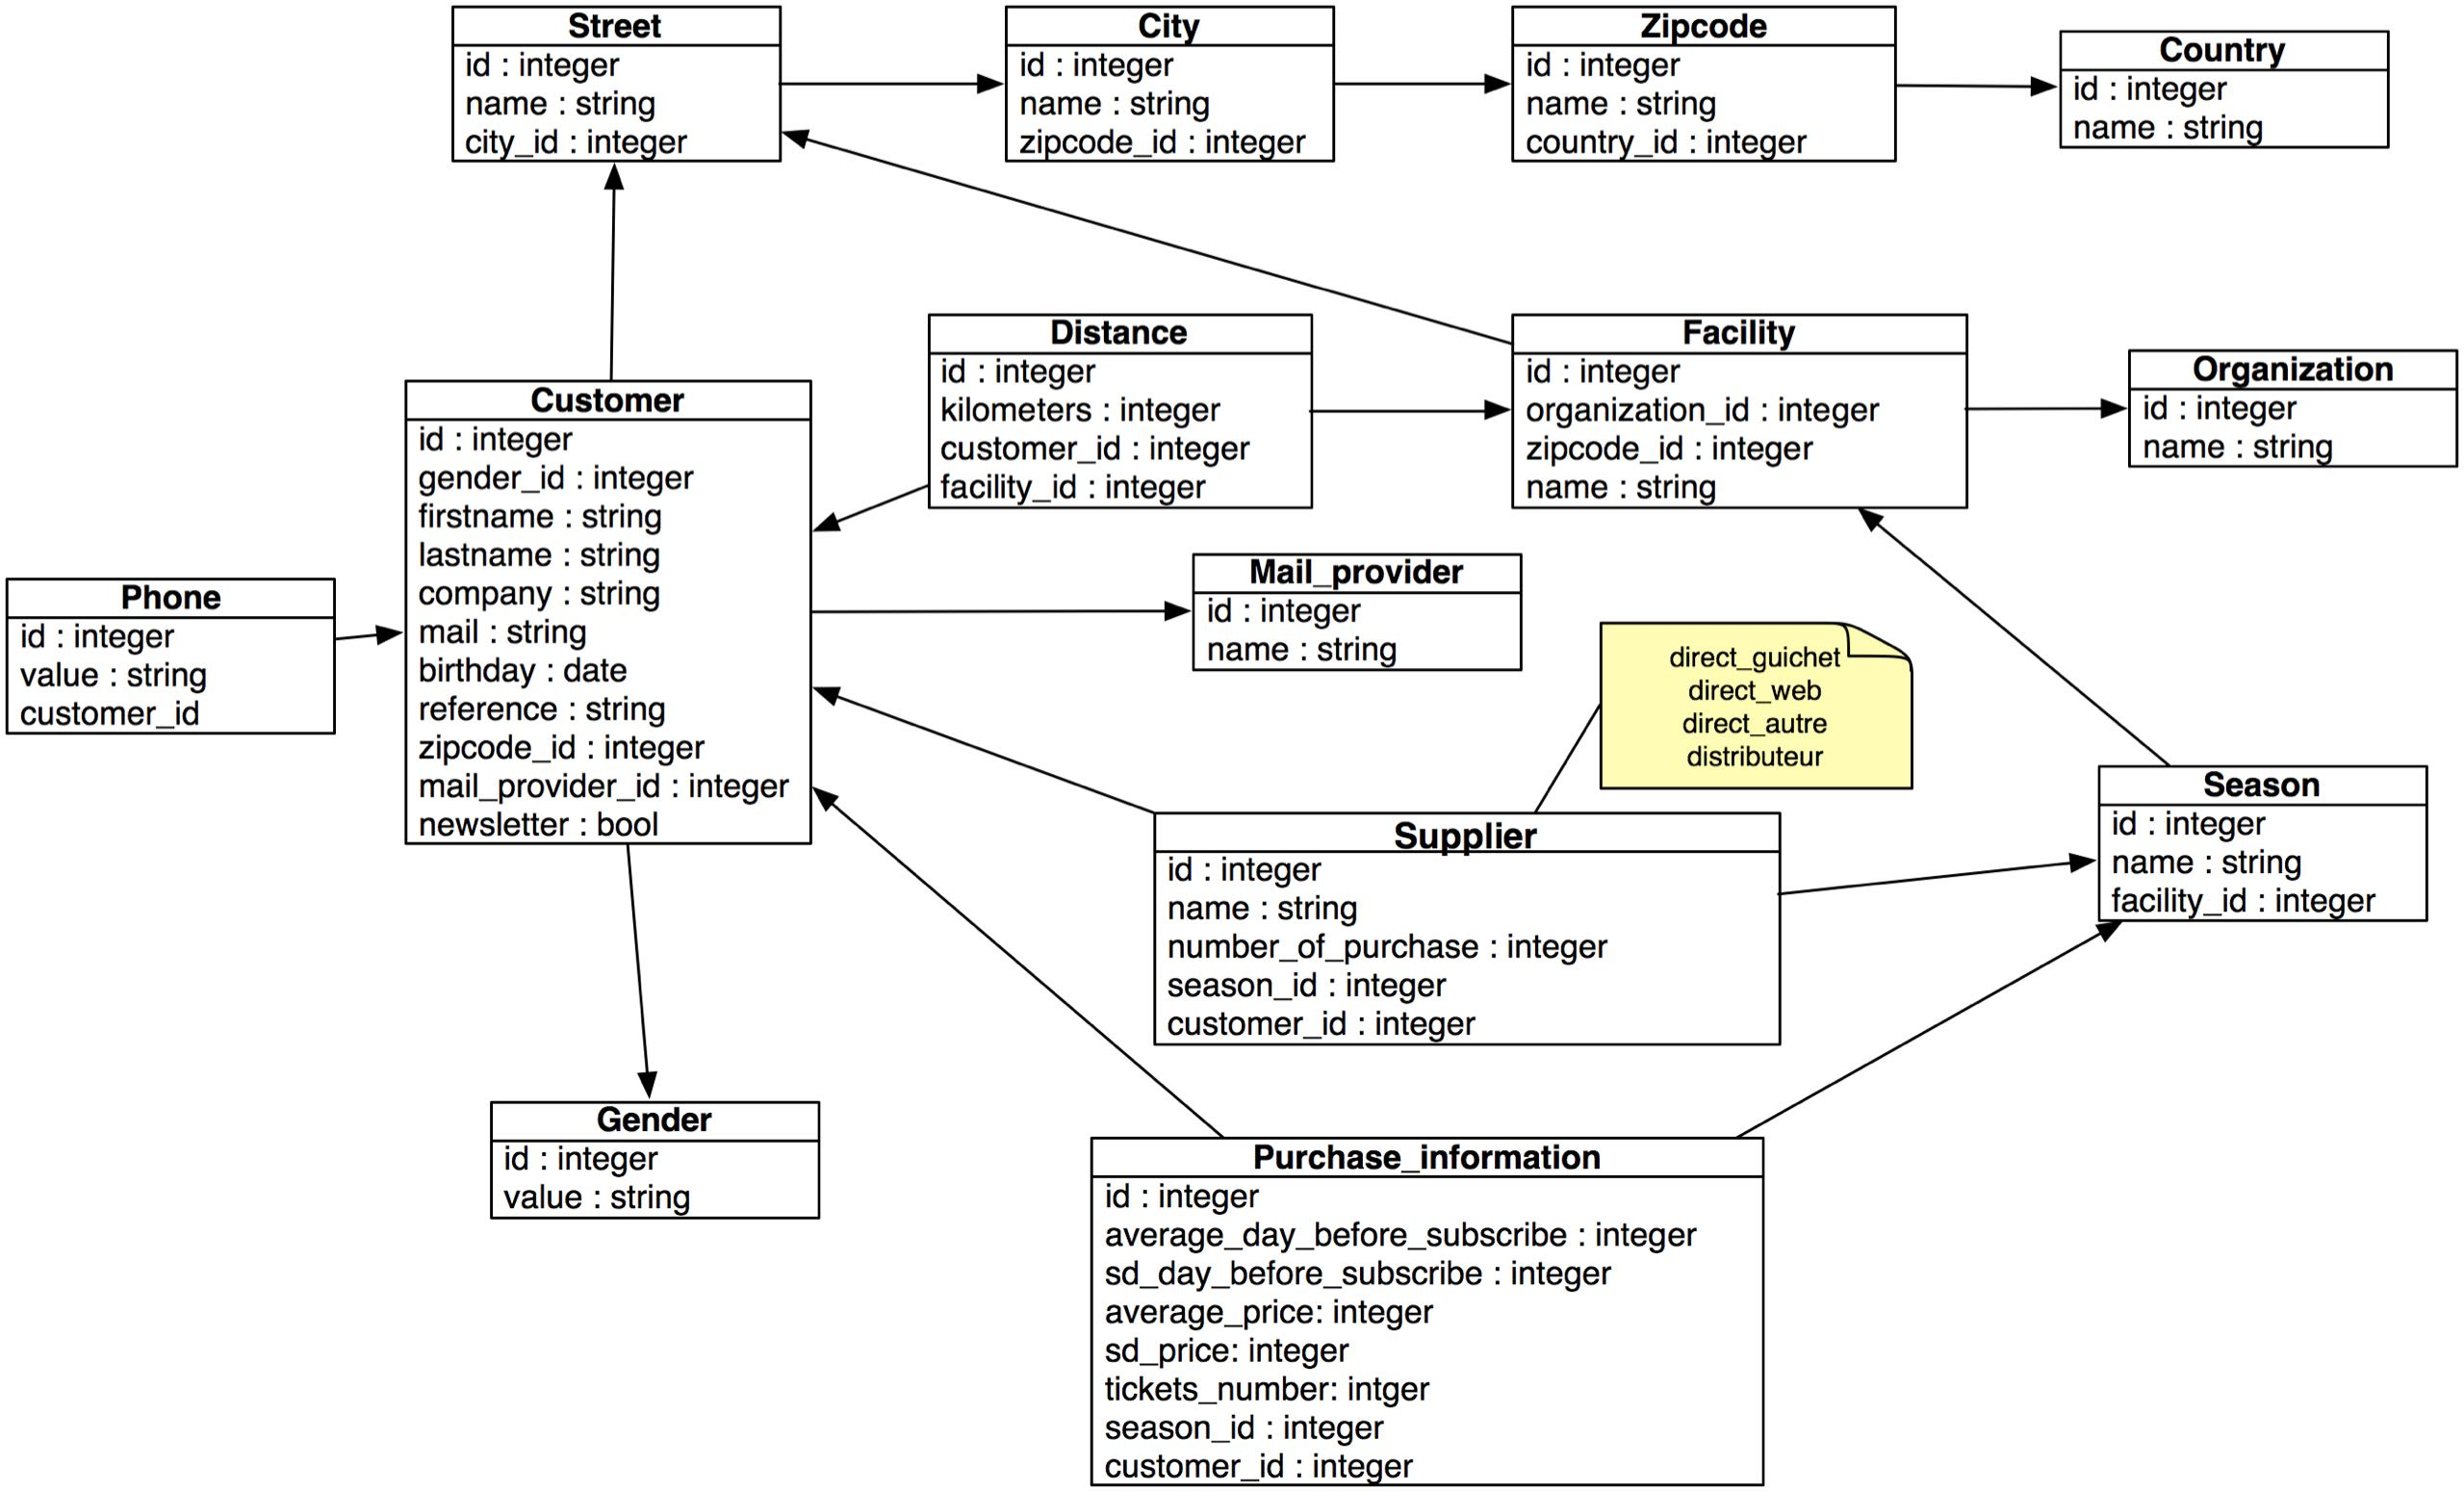
\includegraphics[scale=0.2]{images/arenapublic-1.jpg}
\captionof{figure}{Premiere architecture de la base de données ArenPublic}
\label{arenapublic-1}
\end{center}


Comme le montre l'architecture de base de données \ref{arenapublic-1} page \pageref{arenapublic-1} des données comme des écarts types et des moyennes dans les tables "Supplier" et "Purchase information" sont calculées à la volé et utilisés par les statisticiens. Le problème est qu'il nous faut pouvoir ajouter de nouvelles données facilement en fonction de la demande du client ou du besoin des statisticiens.
\\

Nous décidons donc d'utiliser en complément de la base de donnée SQL une base de base de données de type NoSQL \footnote{Not only SQL} qui permet de rajouter des informations "à la volée" sans modifier la structure de la base de données. 

\subsection{Implémentation technique}
Pour la base de données NoSQL nous voulions uns solution simple à mettre d’oeuvre de type clé valeur. Nous utilisons donc le système de base de données décentralisée Riak qui permet de stocker des informations de type clé valeur dans un bucket.

\begin{center}
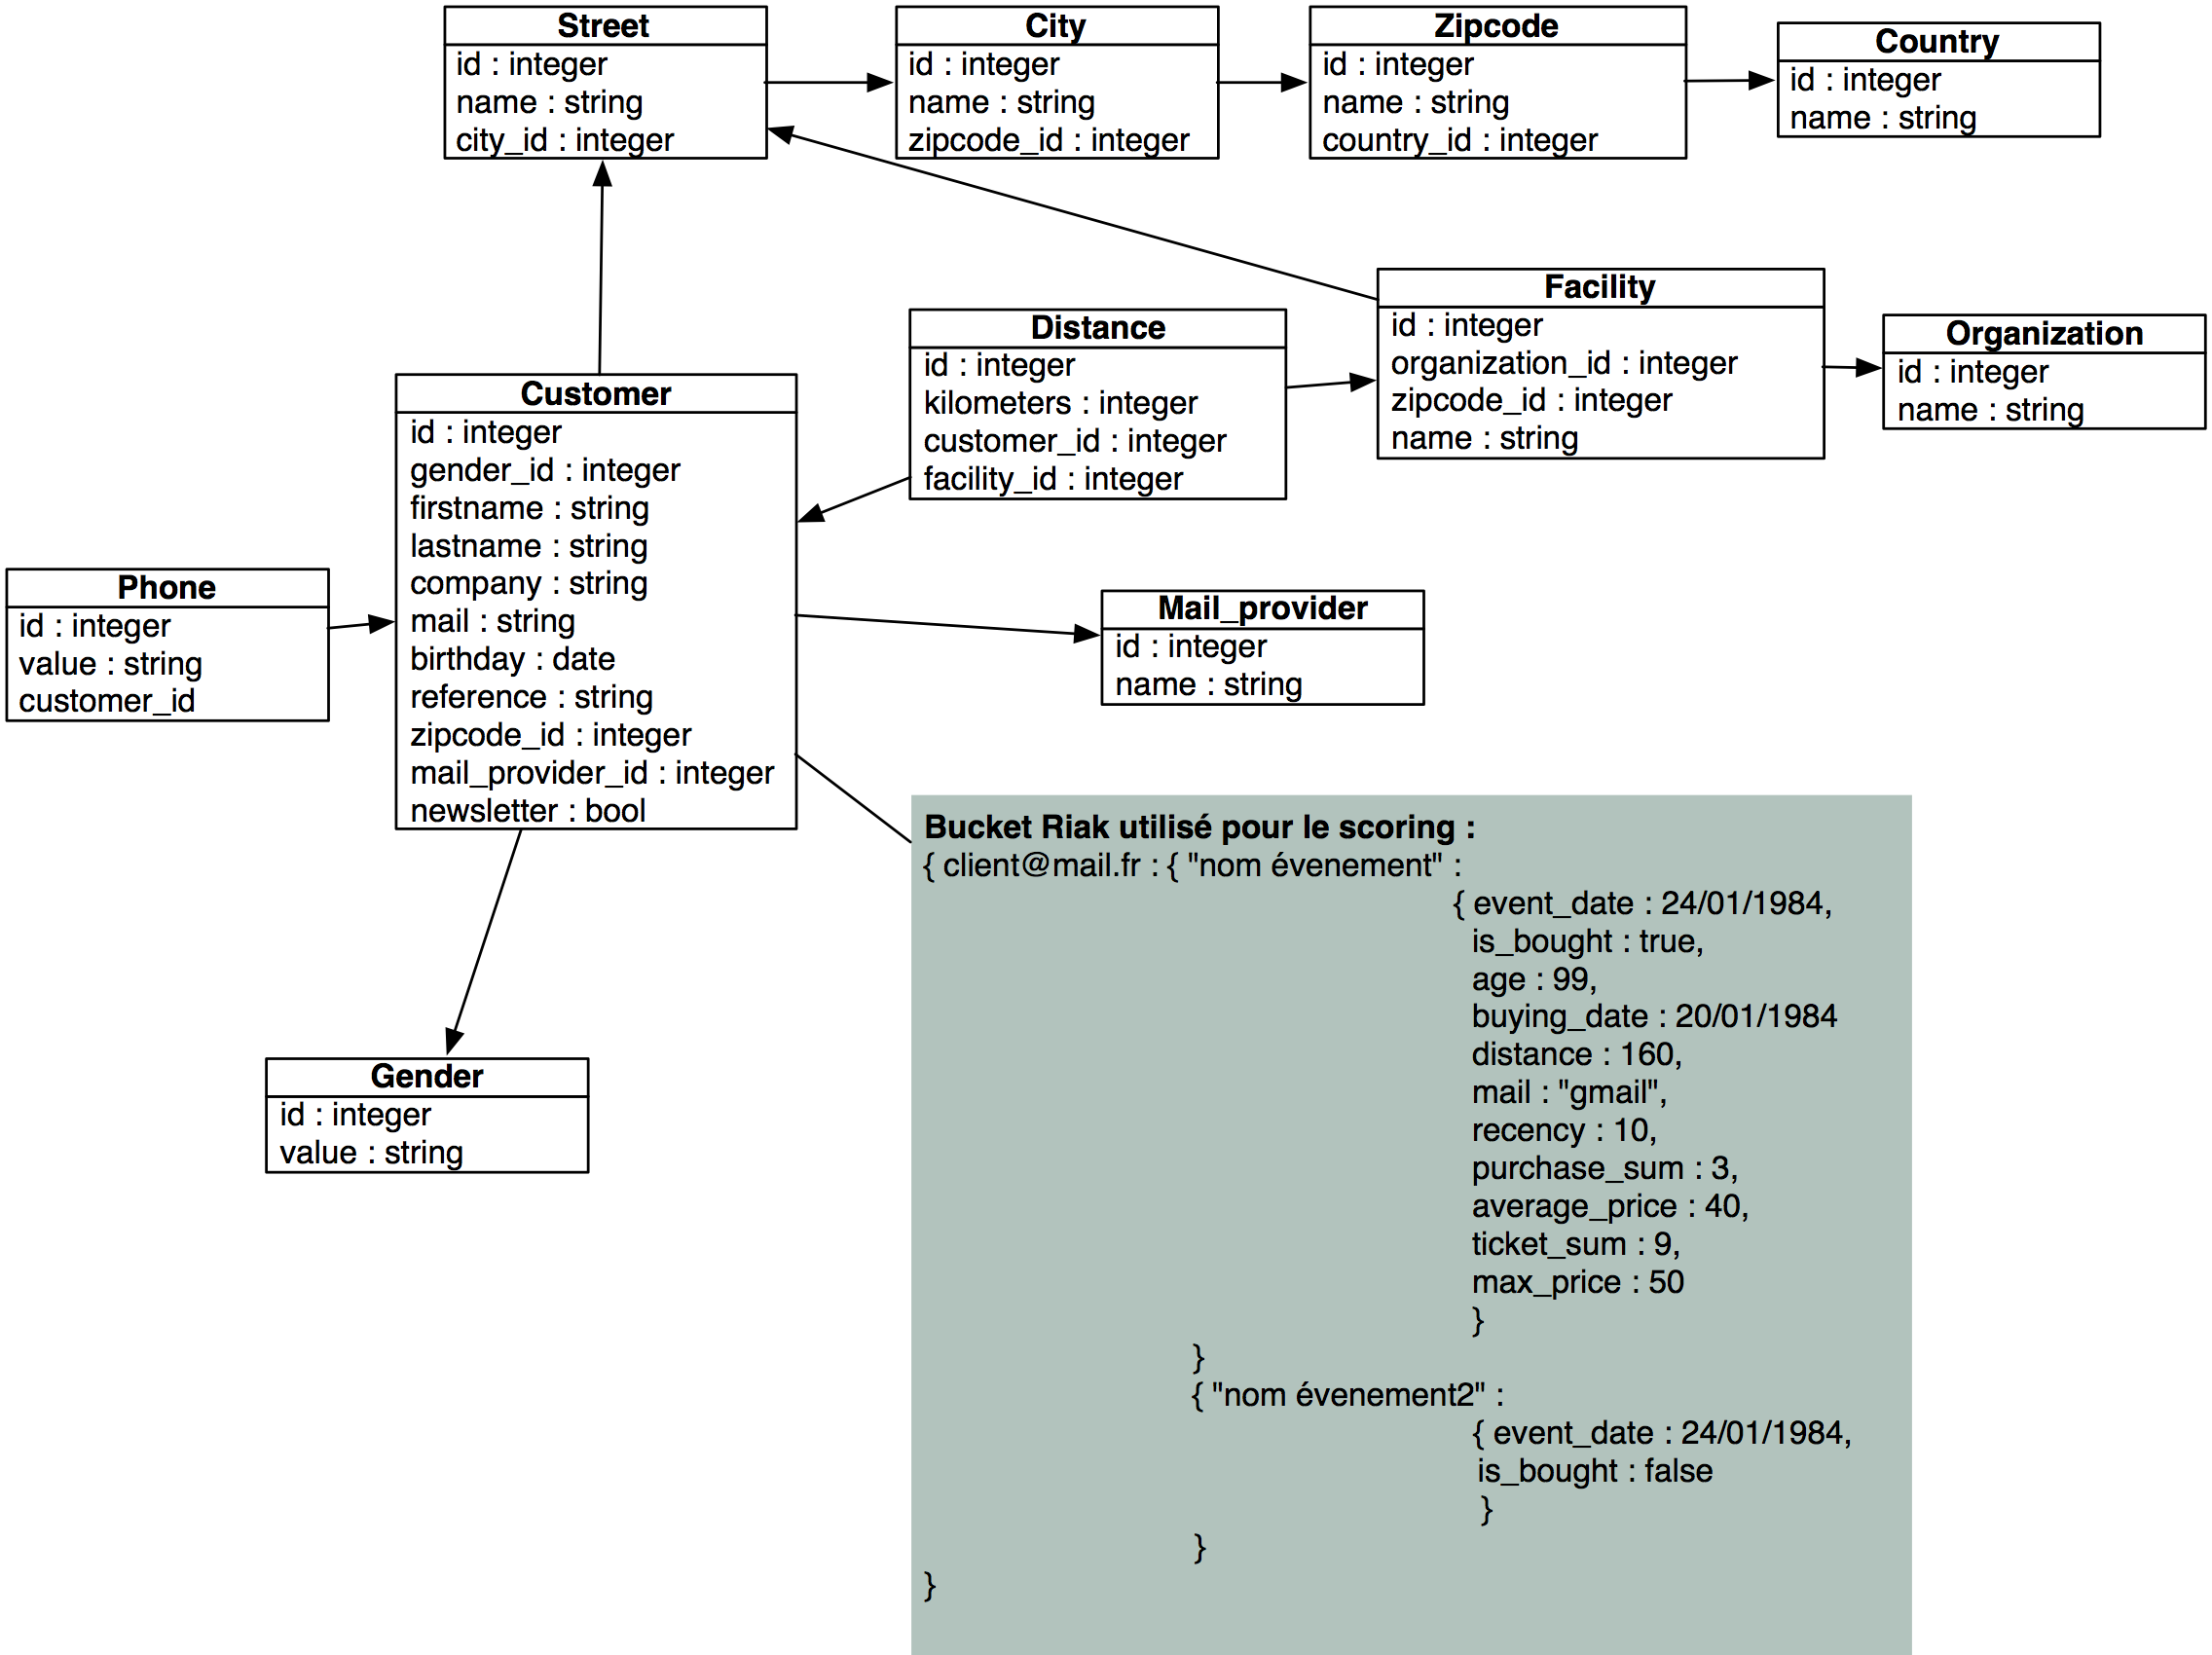
\includegraphics[scale=0.62]{images/arenapublic-2.png}
\captionof{figure}{Architecture finale de la base de données ArenaPricing}
\label{arenapublic-2}
\end{center}

Finalement nous obtenons l'architecture de base de données visible en \ref{arenapublic-2} page \pageref{arenapublic-2}.

La clé du Riak est l'adresse mail du client dans la base de données, il s'agit de la seule valeur vraiment indispensable pour identifier les clients de manière unique.

\subsection{Remplissage de la base de données}

Pour remplir la base de données ArenaPublic nous pouvons utiliser deux méthodes : 
\begin{itemize}
  \item[\textbullet] Un front d'upload qui permet d'envoyer un fichier CSV avec les clients abonnés pour une saison spécifique.
  \item[\textbullet] En allant piocher directement dans la base de données ArenaPricing.
  \end{itemize} \
  
\begin{center}
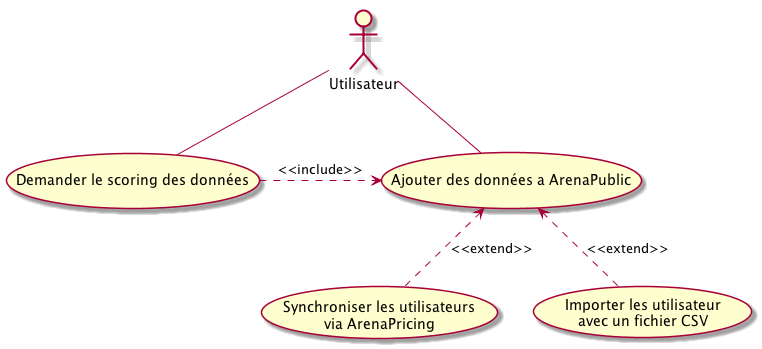
\includegraphics[scale=0.6]{images/arenapublic-use-case.png}
\captionof{figure}{Diagramme des cas d'utilisation de ArenaPublic}
\label{arenapublic_use_case}
\end{center}

Le diagramme des cas d'utilisation \ref{arenapublic_use_case} page \pageref{arenapublic_use_case} montre les différentes possibilités pour l'utilisateur d'importer des données relatives aux consommateurs afin de les scorer.
\begin{itemize}
	\item[\textbullet] Synchronisation des données depuis ArenaPricing 
	\item[\textbullet] Importation des données depuis un fichier CSV 
\end{itemize}
\leavevmode \\

Pour ma part j'ai essentiellement travaillé sur la synchronisation et l'agrégation des données depuis ArenaPricing. 
\\

Pour faire cela j'ai utilisé le langage Python, car il permet de facilement gérer des dictionnaires et de nombreux modules mathématiques sont disponibles pour pour fournir au statisticien des données aussi complètes que possible. Il ne leur reste ainsi qu'à les analyser.

\begin{center}
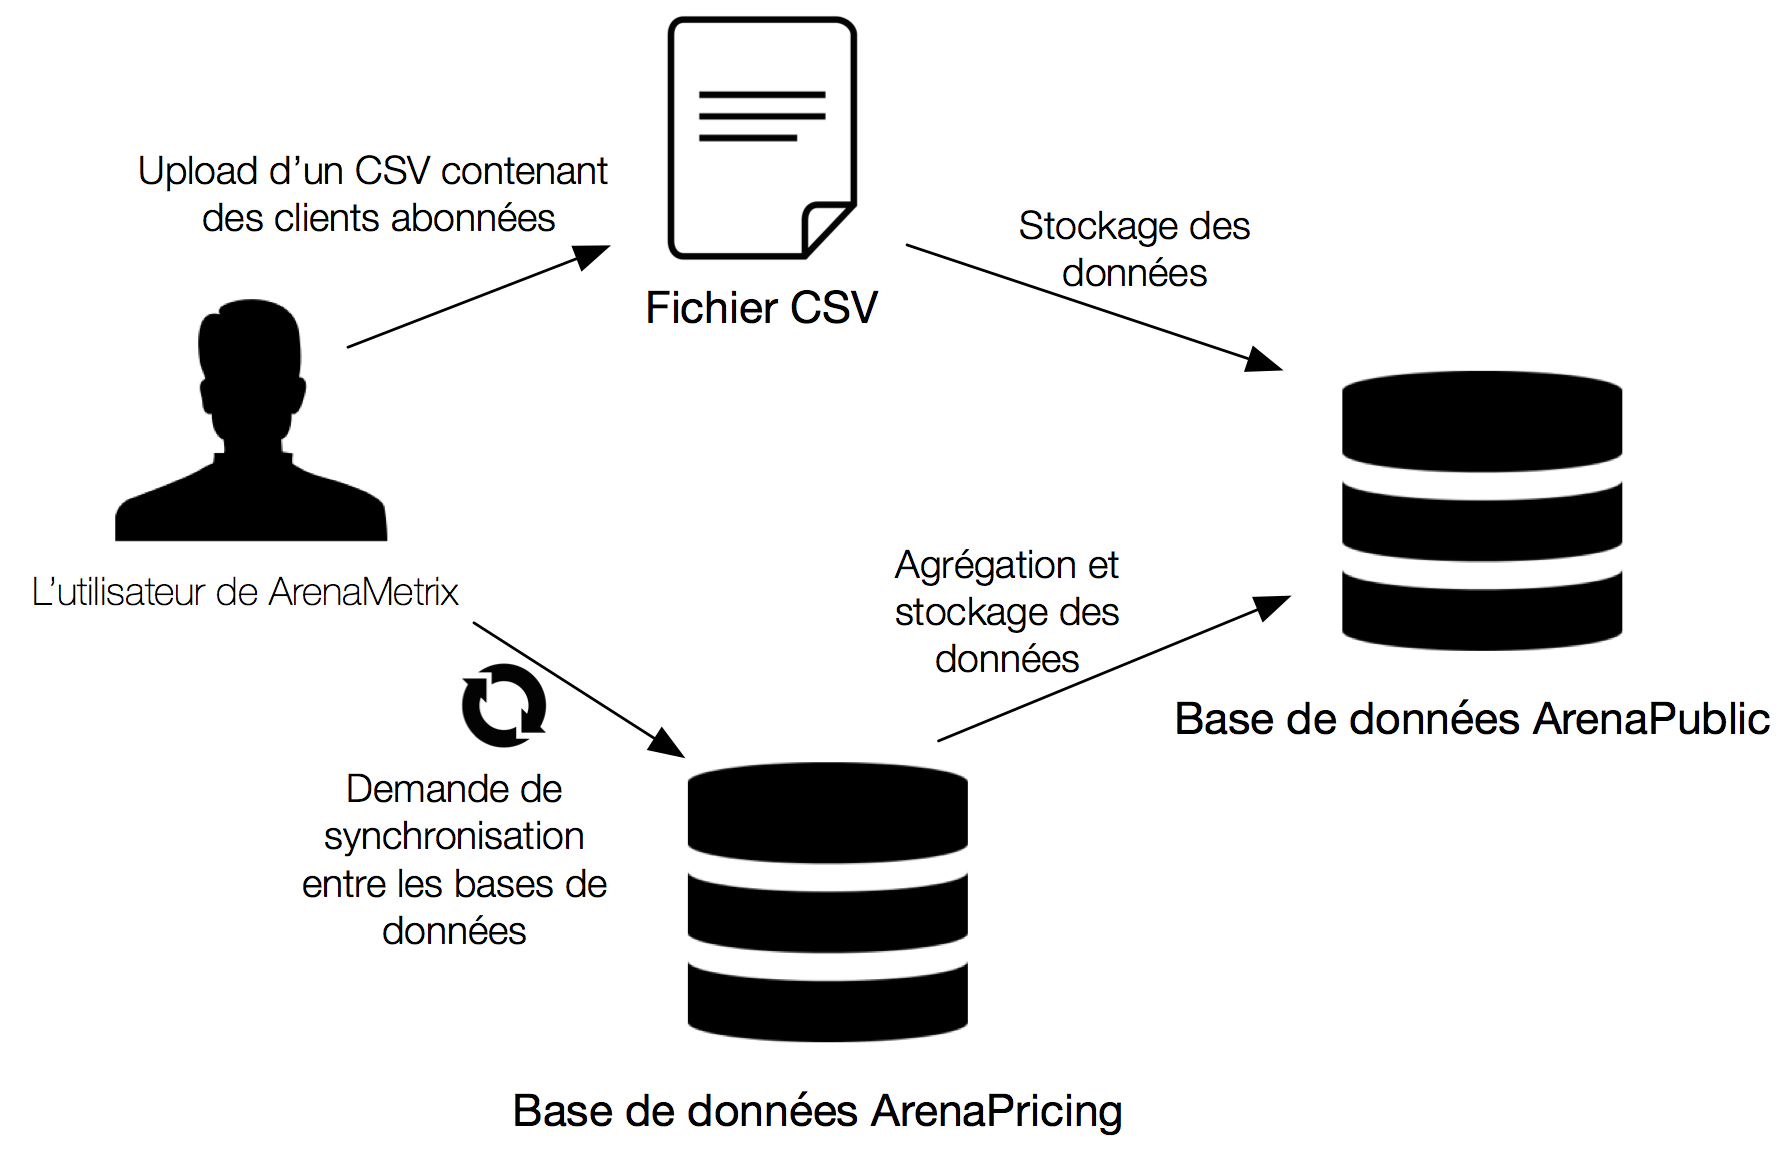
\includegraphics[scale=0.7]{images/public-to-pricing.png}
\captionof{figure}{Remplissage de la base de données ArenaPicing}
\label{public-to-pricing}
\end{center}

Comme le montre la figure \ref{public-to-pricing} page \pageref{public-to-pricing} il est possible pour l'utilisateur d'envoyer ses données au choix depuis un fichier CSV ou en synchronisant les données avec la base de données ArenaPricing. 
\\

La synchronisation des données avec ArenaPricing permet la réalisation d'un CRM à partir de données billéterie, d'un point de vue commercial ArenaPublic est uniquement disponibles pour le client ayant souscrit aux deux offres. 
\\

Tech4Team propose ainsi deux offres de scoring différentes : 

\begin{itemize}
  \item[\textbullet] Scoring sur le réabonnement : pour les clients nous fournissant des données abonnées. 
  \item[\textbullet] Scoring sur l'achat : pour les clients ayant des données dans ArenaPricing  
\end{itemize} 



\subsection{Enrichissement des données}
Lors de l'agrégation des données de ArenaPricing dans ArenaPublic en plus de faire les calculs servant aux statisticiens, j'ai enrichi les données disponibles afin d'offrir plus de possibilités au statisticien.
\subsubsection{Détermination du sexe}
Ajout du sexe de la personne en fonction du prénom lorsque l'information n'est pas disponible :
our réaliser cet enrichissement de données, j'ai utilisé le module 
\href{https://github.com/ferhatelmas/sexmachine/}{SexMachine}
Ce module retourne male, female, mostly\_male, mostly\_female ou andy en fonction du prénom passe en paramètre.

\lstset{style=custompython}
\begin{lstlisting}
>> import sexmachine.detector as gender
>>> d = gender.Detector()
>>> d.get_gender(u"Bob")
u'male'
>>> d.get_gender(u"Sally")
u'female'
>>> d.get_gender(u"Pauley") # should be androgynous
u'andy'
\end{lstlisting}
\captionof{lstlisting}{Exemple d'utilisation de SexMachine}
\leavevmode \\
Le problème avec le module officiel de SexMachine répertorié sur pypi est qu'il est compatible uniquement avec la version 2.7 de Python. Hors nous utilisons Python 3.X pour l'ensemble de nos logiciels et scripts Python. 

J'ai donc modifié SexMachine pour le rendre compatible avec Python 3.X. Le code source de la version modifié est disponible sur mon repository Github : \href{https://github.com/ludovicl/sexmachine}{https://github.com/ludovicl/sexmachine}.

\subsubsection{Calcul de la distance}

Pour enrichir les données des clients nous calculons la distance entre l'adresse de l'acheteur et l'adresse de l'infrastructure où a lieu l'événement.
Pour faire cela, j'utilise le module geocoder qui permet de wrapper différents sites de géocoding.
\\ \\
Après plusieurs tests j'utilise l'API de tomtom, car elle me donne les meilleurs résultats pour la France et n'a pas de limite d'utilisation.

\lstset{style=custompython}
\begin{lstlisting}
>>> import geocoder
>>> location_customer = geocoder.tomtom('Paris')
>>> location_facility = geocoder.tomtom('12 Rue Thierry Mieg, Belfort')
>>> geocoder.distance(location_customer, location_facility)
359.0865720640995
\end{lstlisting}
\captionof{lstlisting}{Exemple d'utilisation de geocoder}
\leavevmode \\

\subsection{Implémentation de bout en bout}
Pour faire communiquer nos applications de bout en bout nous utilisons MessagePack : il s'agit d'un format de sérialisation binaire qui permet d'échanger des données comme en JSON.

Ainsi, comme le montre le diagramme \ref{scoring} page \pageref{scoring} pour le scoring : 

\begin{itemize}
  \item[\textbullet] Le client demande la synchronisation de sa base de données ticket ArenaPricing en cliquant sur un bouton
  \item[\textbullet] L'interface (Ruby on Rails) lance une requête put une URL d'écoute qui est lancée en Flask depuis DataProc
  \item[\textbullet] DataProc récupère les données d'ArenaPricing, les agréges et les enrichie
  \item[\textbullet] DataProc enregistre les nouvelles données dans les bases de données PostegreSQL et Riak d'ArenaPublic
  \item[\textbullet] Le client est notifié que les données sont maintenant dans ArenaPublic
  \item[\textbullet] Le client sélectionne les données qu'il veut scorer
  \item[\textbullet] Les données sont récupérées dans la base de données
  \item[\textbullet] Les données sont envoyées au logiciel de scoring écris en Python. Le logiciel de scoring écoute sur une URL grâce à une instance lancée en Flask
  \item[\textbullet] Le logiciel de scoring retourne les données à la WebInterface
  \item[\textbullet] La WebInterface unpack le MesagePack et affiche les données associées sous forme de graphiques. 
 

\end{itemize} 

\begin{center}
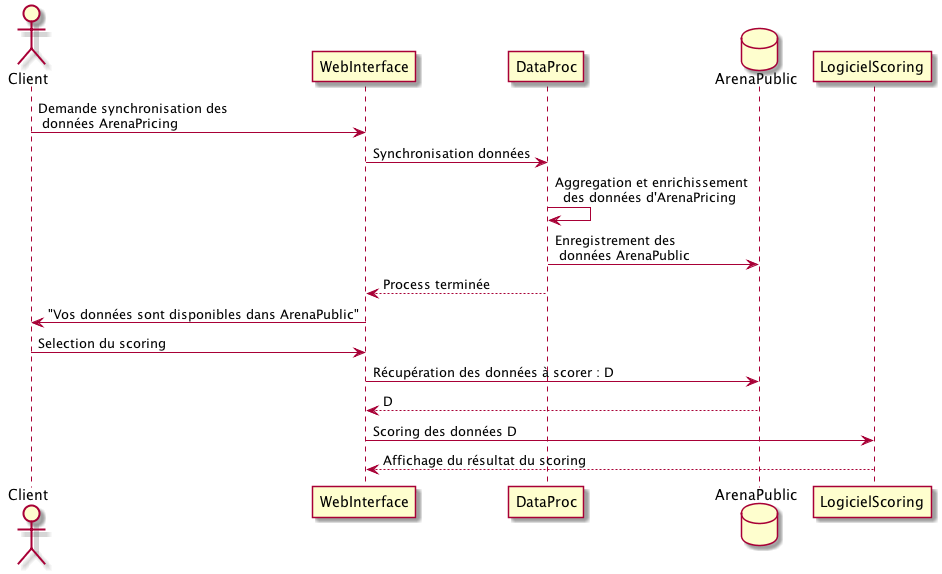
\includegraphics[scale=0.52]{images/scoring.png}
\captionof{figure}{Diagramme de séquence du scoring }
\label{scoring}
\end{center}


\section{Accueil et encadrement de stagiaires}
Début juin de nombreux stagiaires ont été recrutés, ces stagiaires étant en première années de l'ETNA je les ai donc managés et encadrée d'un point de vue technique :
\begin{itemize}
	\item[\textbullet] J'ai notamment eu sous ma responsabilité directe un stagiaire back-end qui a travaillé sur du Python et qui a fait la partie récupération des données exogènes comme la météo et le scrapping de certains sites. 
	\item[\textbullet] Un autre stagiaire était chargé de faire le front-end de ArenaPublic, j'ai donc direcemnt travaillé avec lui car je m'occupai de la partie Python et back-end Ruby de ce projet. Je l'ai également aidé pour les requêtes SQL à effectuer.
\end{itemize}

  


